
\subsection{Comparison with other approaches.}

In this section, we will conduct a comparative analysis of the proposed complete coverage path planning (CCP) algorithm against two alternative approaches: the lawnmower approach, which serves as the baseline for this thesis, and the graph search approach. The comparison will be conducted under the same experimental conditions described in the simulation section without considering the obstacles, utilizing identical datasets and performance metrics to ensure consistency and fairness in evaluation.

\vspace*{6mm}   

Simulation Setup

As with the initial simulations, the setup is designed to emulate the operational environment of an agricultural field. The same datasets used in the evaluation of the proposed CCP algorithm will be employed here to facilitate a direct comparison. These datasets are characterized by different point distributions and densities, ensuring a comprehensive assessment of each approach’s performance.

\vspace*{6mm}   

The key performance metrics for comparison include computational time, field operation time, route length, and energy consumption. These metrics will provide a detailed view of each algorithm's efficiency, effectiveness, and overall robustness.

\vspace*{6mm}   

Lawnmower Approach:


The lawnmower approach, often referred to as the boustrophedon path, is a widely used baseline method in coverage path planning. It involves the robot traversing the field in parallel lines, akin to a lawnmower, ensuring that the entire area is covered systematically. This method is straightforward but may not be optimal in terms of path length and energy consumption, particularly in fields with irregular plant distributions or obstacles.

\vspace*{6mm}   

Graph Search Approach
The graph search approach utilizes a graph-based representation of the field, where points of interest (weeds and cluster of weeds, in this context) are treated as nodes, and paths between them are edges. Algorithms such as A* or Dijkstra's can be employed to find an optimal path that covers all nodes following the non-holonomic constraints. However, this apprach does not guarantee prioritization of approximate straight paths but respects the non-holonomic constraints.  


\vspace*{6mm}   

Performance Metrics


The performance metrics for all datasets and approaches will be summarized in the (\autoref{tab:comparison_table}). These metrics will provide a comprehensive view of each algorithm's performance under different scenarios, enabling a detailed comparison of their efficiency and effectiveness. The results will be analyzed to identify the strengths and weaknesses of each approach, facilitating an informed decision on the most suitable method for complete coverage path planning in agricultural fields.


\begin{table}[htbp]
    \centering
    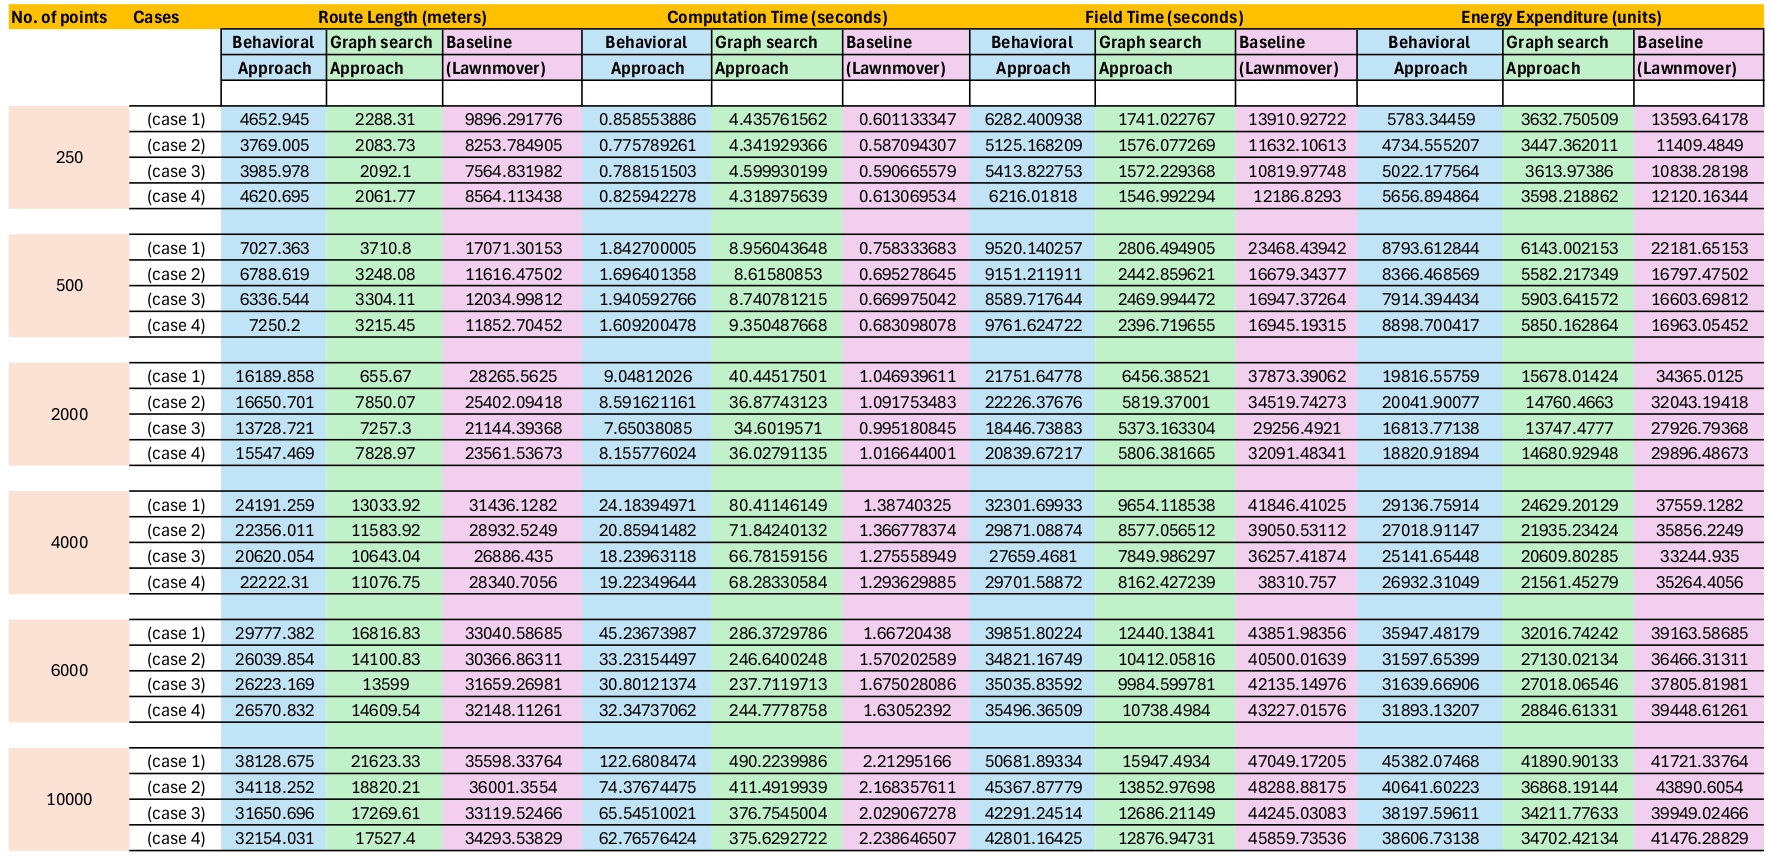
\includegraphics[width=\textwidth]{experimental_data/new_table_image.png}
    \caption{Performance metrics for comparison of all approaches.}
    \label{tab:comparison_table}
\end{table}


\vspace*{6mm}

The lawnmover approach and behavioral approach was performed on the same device. However, the graph search approach was performed on a different device with the following specifications:
11th Gen Intel(R) Core(TM) i7-1165G7 @ 2.80GHz

8 Cores

32GB RAM

\vspace*{6mm}

% write that, we will display the resutls of each approach as plots for each metric separately.


The results of the comparison among the proposed behavioral algorithm, the lawnmower approach, and the graph search approach are presented in the following plots ((\autoref{fig:Computation_time_all}), (\autoref{fig:Energy_expenditure_all}), (\autoref{fig:Route_length_all}), and (\autoref{fig:Field_operation_time_all})). Each plot represents a specific performance metric, such as computational time, energy consumption, route length, and field operation time for all the datasets. 

\begin{figure}[H]
    \centering
    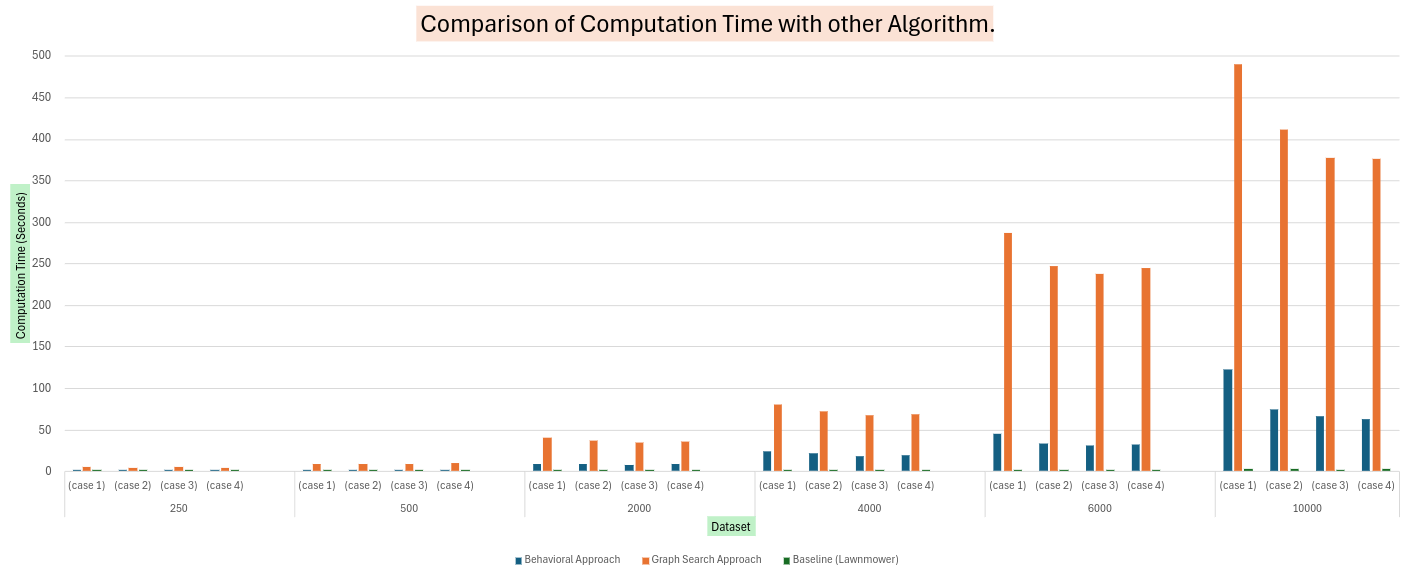
\includegraphics[width=\textwidth]{Images/plots/all/Computation_time.png}
    \caption{Computation Time.}
    \label{fig:Computation_time_all}
\end{figure}

\begin{figure}[H]
    \centering
    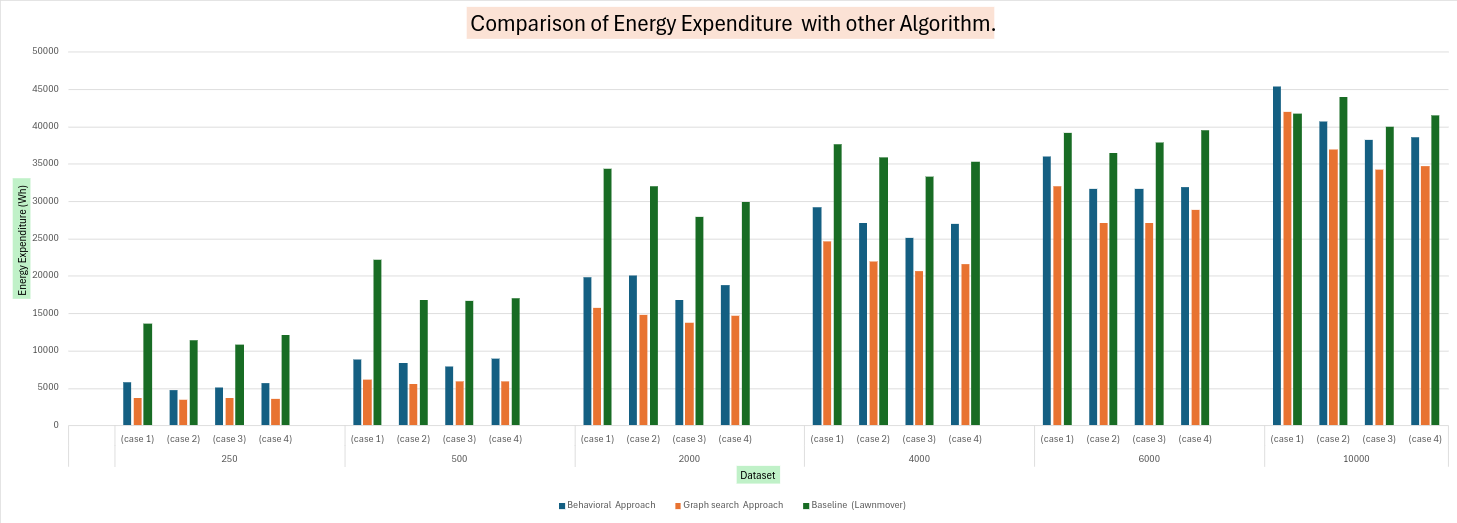
\includegraphics[width=\textwidth]{Images/plots/all/Energy.png}
    \caption{Energy Expenditure.}
    \label{fig:Energy_expenditure_all}
\end{figure}

\begin{figure}[H]
    \centering
    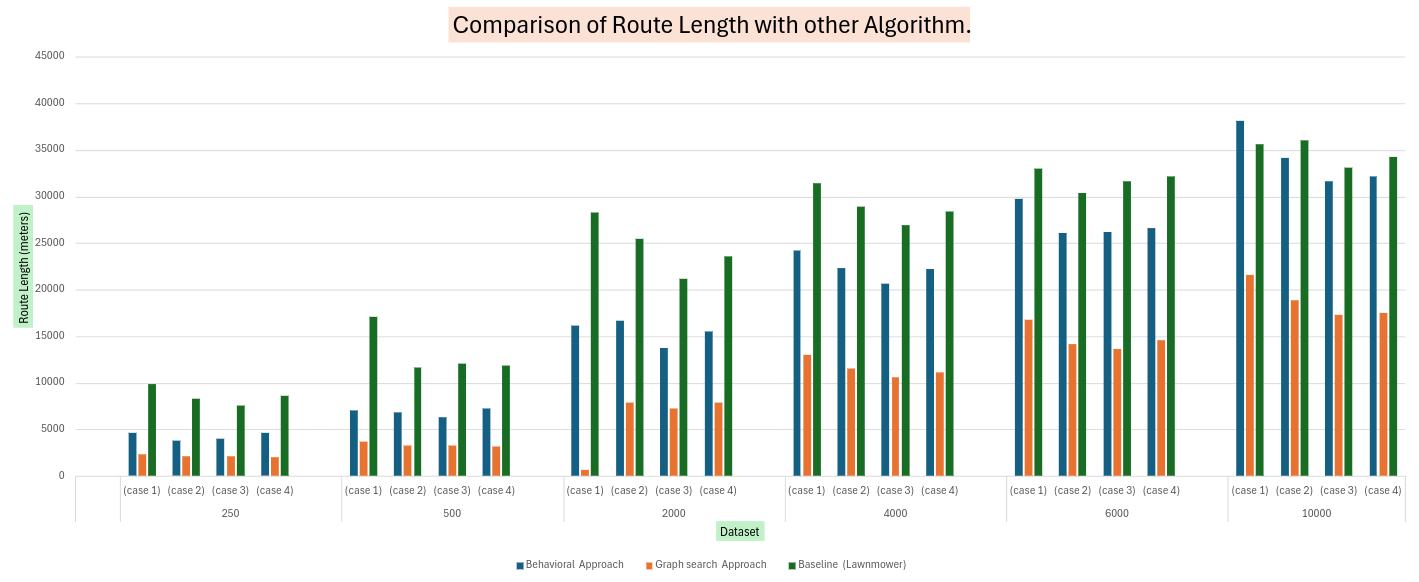
\includegraphics[width=\textwidth]{Images/plots/all/route_length.png}
    \caption{Route Length.}
    \label{fig:Route_length_all}
\end{figure}

\begin{figure}[H]
    \centering
    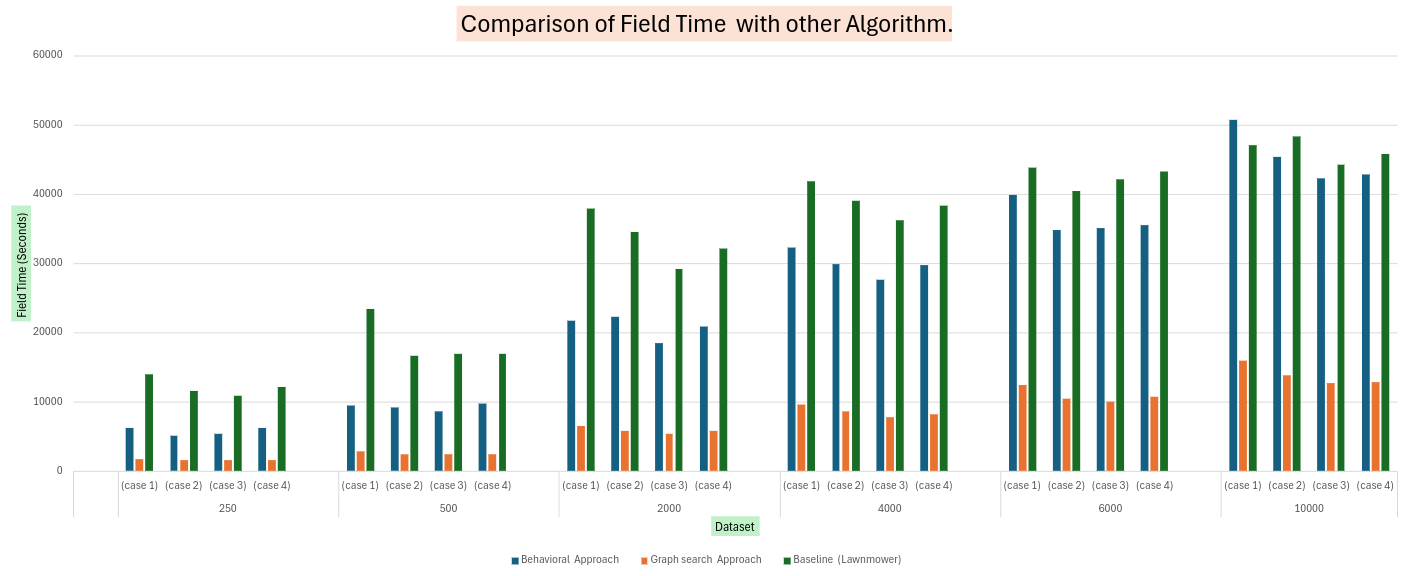
\includegraphics[width=\textwidth]{Images/plots/all/Field_time.png}
    \caption{Field Operation Time.}
    \label{fig:Field_operation_time_all}
\end{figure}


\textbf{Analysis of the comparison results}  


